\documentclass[tikz,border=6pt]{standalone}
\usepackage{tikz}
\usetikzlibrary{positioning,arrows.meta,fit,backgrounds,calc,shapes.geometric,shapes.misc}
\definecolor{cenc}{RGB}{65,105,170}
\definecolor{cdec}{RGB}{195,80,80}
\definecolor{cfreq}{RGB}{240,160,60}
\definecolor{ctext}{RGB}{90,160,90}
\definecolor{ctgfs}{RGB}{150,90,180}
\definecolor{cll}{RGB}{70,130,180}
\definecolor{chh}{RGB}{200,120,80}

\begin{document}
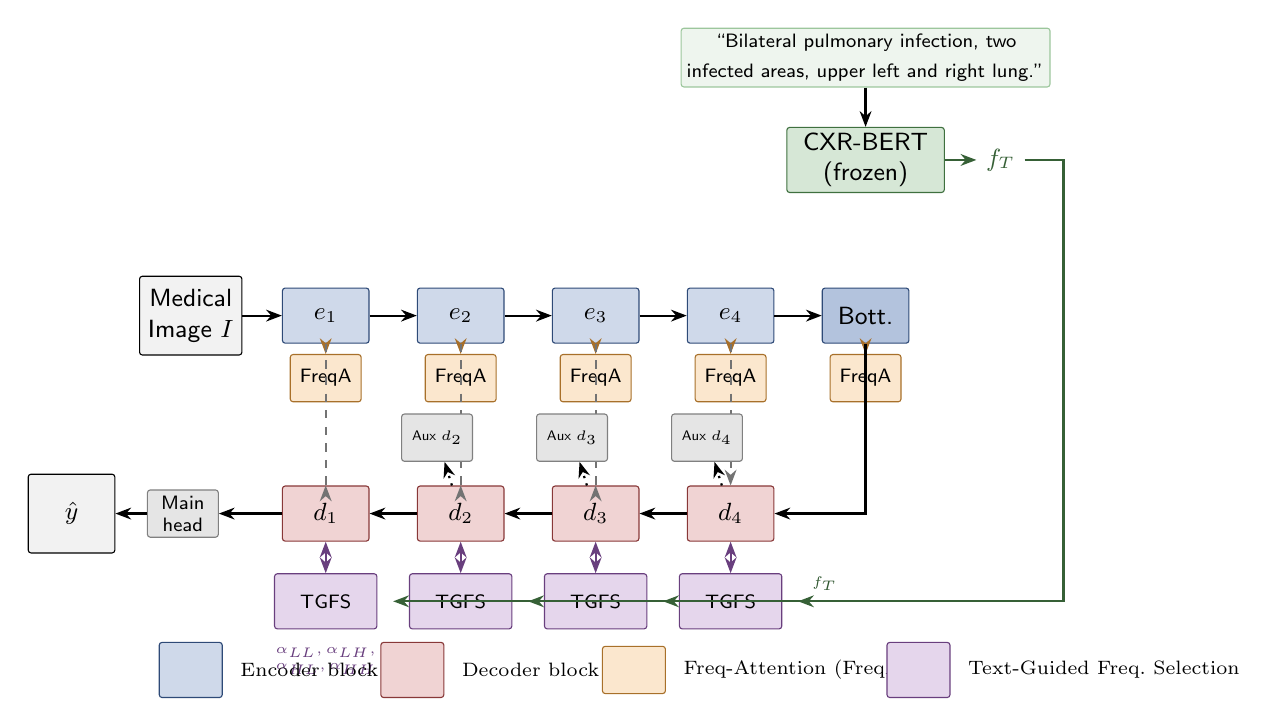
\begin{tikzpicture}[
  node distance=5mm and 6mm,
  font=\sffamily\small,
  >={Stealth[length=2mm]},
  block/.style={rectangle, draw, rounded corners=1pt, minimum height=7mm,
                minimum width=11mm, align=center, inner sep=2pt},
  enc/.style={block, fill=cenc!25, draw=cenc!70!black},
  dec/.style={block, fill=cdec!25, draw=cdec!70!black},
  freq/.style={block, fill=cfreq!25, draw=cfreq!70!black,
               minimum width=9mm, minimum height=6mm, font=\sffamily\scriptsize},
  txtbox_unused/.style={block, fill=ctext!25, draw=ctext!70!black},
  tgfs/.style={block, fill=ctgfs!25, draw=ctgfs!70!black,
               minimum width=13mm},
  head/.style={block, fill=black!10, draw=black!50, minimum width=9mm,
               minimum height=6mm, font=\sffamily\scriptsize},
  arr/.style={->, thick},
  skip/.style={->, thick, dashed, color=black!55},
  txtbox/.style={block, fill=ctext!25, draw=ctext!70!black}
]

% ---------- input image ----------
\node[block, minimum width=13mm, minimum height=10mm, fill=black!5]
  (img) {Medical\\Image $I$};

% ---------- encoder stack ----------
\node[enc, right=5mm of img]             (e1) {$e_1$};
\node[enc, right=of e1]                  (e2) {$e_2$};
\node[enc, right=of e2]                  (e3) {$e_3$};
\node[enc, right=of e3]                  (e4) {$e_4$};
\node[enc, right=of e4, fill=cenc!40]    (bn) {Bott.};

\draw[arr] (img) -- (e1);
\foreach \a/\b in {e1/e2,e2/e3,e3/e4,e4/bn}
  \draw[arr] (\a) -- (\b);

% FreqA labels under each encoder block
\foreach \n in {e1,e2,e3,e4,bn}
  \node[freq, below=1.3mm of \n] (\n f) {FreqA};
\foreach \n in {e1,e2,e3,e4,bn}
  \draw[->, thin, color=cfreq!70!black] (\n) -- (\n f);

% ---------- decoder stack (below encoder, aligned) ----------
\node[dec, below=18mm of e4] (d4) {$d_4$};
\node[dec, left=of d4]       (d3) {$d_3$};
\node[dec, left=of d3]       (d2) {$d_2$};
\node[dec, left=of d2]       (d1) {$d_1$};

% bottleneck to d4
\draw[arr] (bn) |- (d4);

\foreach \a/\b in {d4/d3,d3/d2,d2/d1}
  \draw[arr] (\a) -- (\b);

% skip connections: encoder -> decoder
\draw[skip] (e4) -- ++(0,-6mm) -| (d4.north);
\draw[skip] (e3) |- (d3.north);
\draw[skip] (e2) |- (d2.north);
\draw[skip] (e1) |- (d1.north);

% ---------- text branch ----------
\node[txtbox, above=12mm of bn, minimum width=20mm, align=center]
  (bert) {CXR-BERT\\(frozen)};
\node[block, fill=ctext!10, draw=ctext!60, above=of bert,
      minimum width=42mm, align=center]
  (rep) {\scriptsize ``Bilateral pulmonary infection, two\\
                     \scriptsize infected areas, upper left and right lung.''};
\draw[arr] (rep) -- (bert);

% text embedding output arrow
\node[right=4mm of bert, color=ctext!60!black] (ftsrc) {$f_T$};
\draw[arr, color=ctext!60!black] (bert.east) -- (ftsrc);

% ---------- TGFS modules ----------
\node[tgfs, below=4mm of d4] (t4) {\scriptsize TGFS};
\node[tgfs, below=4mm of d3] (t3) {\scriptsize TGFS};
\node[tgfs, below=4mm of d2] (t2) {\scriptsize TGFS};
\node[tgfs, below=4mm of d1] (t1) {\scriptsize TGFS};

\foreach \d/\t in {d4/t4,d3/t3,d2/t2,d1/t1}
  \draw[<->, thick, color=ctgfs!70!black] (\d) -- (\t);

% text -> TGFS (bus)
\coordinate (textbus) at ($(ftsrc)+(8mm,0)$);
\draw[arr, color=ctext!60!black] (ftsrc) -- (textbus) |- ($(t4.east)+(2mm,0)$)
       node[pos=0.95, above, font=\tiny, color=ctext!55!black] {$f_T$};
\draw[arr, color=ctext!60!black] (textbus) |- ($(t3.east)+(2mm,0)$);
\draw[arr, color=ctext!60!black] (textbus) |- ($(t2.east)+(2mm,0)$);
\draw[arr, color=ctext!60!black] (textbus) |- ($(t1.east)+(2mm,0)$);

% ---------- gate output annotations under one TGFS ----------
\node[below=1mm of t1, font=\tiny, color=ctgfs!70!black, align=center]
  (gates) {$\alpha_{LL},\alpha_{LH},$\\$\alpha_{HL},\alpha_{HH}$};

% ---------- heads ----------
\node[head, left=8mm of d1]   (head1) {Main\\head};
\node[head, above=3mm of d4, xshift=-3mm]  (aux4) {\tiny Aux $d_4$};
\node[head, above=3mm of d3, xshift=-3mm]  (aux3) {\tiny Aux $d_3$};
\node[head, above=3mm of d2, xshift=-3mm]  (aux2) {\tiny Aux $d_2$};
\draw[arr] (d1) -- (head1);
\draw[arr, dotted] (d4) -- (aux4);
\draw[arr, dotted] (d3) -- (aux3);
\draw[arr, dotted] (d2) -- (aux2);

% output
\node[block, left=4mm of head1, fill=black!5, minimum height=10mm] (mask) {$\hat{y}$};
\draw[arr] (head1) -- (mask);

% ---------- legend ----------
\begin{scope}[shift={(0,-4.5)}]
 \node[enc, minimum width=8mm]              (le)  at (0,0) {};
 \node[right=1mm of le, font=\scriptsize]         {Encoder block};
 \node[dec, minimum width=8mm, right=20mm of le]  (ld) {};
 \node[right=1mm of ld, font=\scriptsize]         {Decoder block};
 \node[freq, minimum width=8mm, right=20mm of ld] (lf) {};
 \node[right=1mm of lf, font=\scriptsize]         {Freq-Attention (FreqA)};
 \node[tgfs, minimum width=8mm, right=28mm of lf] (lt) {};
 \node[right=1mm of lt, font=\scriptsize]         {Text-Guided Freq.\ Selection};
\end{scope}

\end{tikzpicture}
\end{document}
